\documentclass{article}

\usepackage{arxiv}

\usepackage[utf8]{inputenc}
\usepackage[T1]{fontenc}
\usepackage[numbers]{natbib}
\usepackage{hyperref}
\usepackage{url}
\usepackage{booktabs}
\usepackage{amsfonts}
\usepackage{amsmath}
\usepackage{amssymb}
\usepackage{nicefrac}
\usepackage{microtype}
\usepackage{graphicx}
\graphicspath{{figures/}}
\usepackage{xcolor}
\usepackage{algorithm}
\usepackage{algpseudocode}

\title{FitLLM: Adaptive Layer-Sharded Execution for\\ Fine-Tuning and Inference of Large Language Models\\ within Fixed Accelerator-Memory Budgets}

\author{}

\renewcommand{\headeright}{Preprint}
\renewcommand{\undertitle}{Preprint}
\renewcommand{\shorttitle}{FitLLM: Adaptive Layer-Sharded Execution for LLMs}

\hypersetup{
pdftitle={FitLLM: Adaptive Layer-Sharded Execution for Fine-Tuning and Inference of Large Language Models within Fixed Accelerator-Memory Budgets},
pdfsubject={cs.LG, cs.DC},
pdfauthor={},
pdfkeywords={large language models, memory offloading, QLoRA, fine-tuning, speculative decoding},
}

\begin{document}
\maketitle

\begin{abstract}
State-of-the-art large language models (LLMs) routinely exceed the memory
capacity of a single accelerator, forcing practitioners toward multi-GPU
clusters even for parameter-efficient fine-tuning. We present \textbf{FitLLM},
a system that executes both inference and low-rank fine-tuning of large dense
transformers on a single accelerator under a \emph{fixed, user-specified}
VRAM budget---as small as $4$\,GB for a $32$B-parameter model. FitLLM stores
each decoder layer as an independent on-disk shard and streams shards through a
three-stage \mbox{NVMe$\rightarrow$CPU$\rightarrow$accelerator} pipeline, so
that only a small, budget-determined number of layers are resident on the
accelerator at any instant. Three mechanisms make this practical: (i) an
\emph{adaptive multi-shard probe} that re-measures free memory and recomputes
the resident shard width after every batch, degrading gracefully to CPU
execution rather than failing with out-of-memory errors; (ii) a
\emph{reverse-order, shard-wise backward pass} that replays layers from
CPU-resident activation checkpoints and admits a \emph{provable} accelerator
memory ceiling independent of model depth; and (iii) a disk-resident,
per-layer optimizer paired with QLoRA so that only low-rank adapter gradients
are accumulated. We give first-principles analyses of the optimal shard width,
the backward-pass memory bound, and the bandwidth and complexity behaviour of
the accompanying speculative-decoding path with a training-free dynamic draft
controller. We further demonstrate \emph{memory feasibility} empirically: a
$32$B-parameter model is sharded into $64$ per-layer files
($\sim$$15.5$\,GB on disk) and executed forward and backward within a $4$\,GB
working set on a single accelerator, training only $0.10\%$ of parameters.
We discuss the throughput characteristics of the prototype and outline the
remaining engineering required for production-grade end-to-end performance.
\end{abstract}

\keywords{Large language models \and Memory offloading \and Parameter-efficient
fine-tuning \and QLoRA \and Speculative decoding \and Systems for ML}

\section{Introduction}
\label{sec:intro}

The parameter counts of open-weight transformer language models have grown far
faster than the memory of commodity accelerators. A $32$B-parameter model
requires roughly $64$\,GB in \texttt{fp16}, exceeding the capacity of most
single GPUs; a $70$B model in $4$-bit form still requires $\sim$$42$\,GB merely
to hold weights, before activations, key/value (KV) caches, or optimizer state.
The conventional response---data- or tensor-parallel execution across multiple
accelerators---imposes a hardware floor that excludes a large fraction of
practitioners, students, and edge deployments, even when the task is modest
(e.g.\ adapting a model to a domain corpus with a low-rank adapter).

A complementary observation is that a transformer's decoder layers are executed
\emph{sequentially}: during a single forward pass, layer $i$ is needed only
while it is being computed. This invites a \emph{layer-streaming} execution
model in which weights live on cheaper, larger storage tiers (CPU RAM or NVMe)
and are paged onto the accelerator just in time. Existing layer-streaming
systems, however, tend to fix the streaming granularity ahead of time
(e.g.\ one layer at a time, or a static block of $k$ layers), which either
underutilises available memory or risks out-of-memory (OOM) failure when the KV
cache grows during long-context decoding; and they generally target inference
only, leaving on-device fine-tuning unaddressed.

\textbf{FitLLM} is a system for both inference and parameter-efficient
fine-tuning of large dense transformers within a fixed accelerator-memory
budget on a single device. The system organises three memory tiers---NVMe disk,
host RAM, and accelerator VRAM---into a continuously re-balanced pipeline
(\autoref{fig:arch}), and applies the same streaming substrate to the forward
pass, the backward pass, and the optimizer step.

\paragraph{Contributions.} This paper makes the following contributions.
\begin{enumerate}
  \item \textbf{Per-layer disk sharding with integrity.} Each decoder layer is
  serialised to an individual shard file (optionally $4$-bit NF4-quantised) with
  a companion SHA-256 checksum. Sharding is performed once and reused across runs
  and across devices of different capacity (Sections~\ref{sec:overview},
  \ref{sec:impl}).

  \item \textbf{An adaptive multi-shard engine (AMSE).} A lightweight probe reads
  live free accelerator and host memory and recomputes the resident shard width
  $k$ after every batch, selecting one of four execution strategies and
  degrading to CPU rather than crashing when $k\!\to\!0$
  (Section~\ref{sec:amse}).

  \item \textbf{A reverse-order shard-wise backward pass} that replays layers
  from CPU-resident activation checkpoints and accumulates only low-rank adapter
  gradients, with a \emph{provable} accelerator-memory ceiling independent of
  model depth (Section~\ref{sec:backward}).

  \item \textbf{A disk-resident optimizer with QLoRA} that keeps the frozen
  quantised base on disk and the small adapters and their optimizer state in host
  RAM, with a graceful path to full-parameter updates
  (Section~\ref{sec:optim}).

  \item \textbf{First-principles analyses} of optimal shard width, the
  backward-pass memory bound, draft-decoding complexity, optimal speculative
  draft length, and roofline-guided heterogeneous placement
  (Section~\ref{sec:analysis}), plus a memory-feasibility demonstration on a
  $32$B model under a $4$\,GB budget (Section~\ref{sec:eval}).
\end{enumerate}

\paragraph{Scope of claims.} We are explicit about what is established versus
projected. The system architecture and the memory analyses of
Sections~\ref{sec:amse}--\ref{sec:analysis} are exact properties of the
construction. Bandwidth and throughput projections are \emph{analytical} and are
labelled as such; they are not measured benchmarks. Our empirical contribution
(Section~\ref{sec:eval}) is a \emph{feasibility} result: a $32$B model can be
sharded and executed forward and backward within a $4$\,GB working set on a
single accelerator, with the resulting disk footprint and trainable-parameter
ratio reported. We make no convergence or downstream-quality claims; the
dominant overheads of the present prototype and the work required to close them
are analysed in Section~\ref{sec:limitations}. All schematic figures in this
paper illustrate the design; any quantities they show are analytical estimates,
not measured results.

\section{Related Work}
\label{sec:related}

\paragraph{Weight offloading and layer streaming.}
ZeRO-Offload~\citep{ren2021zerooffload} and FlexGen~\citep{sheng2023flexgen}
offload optimizer state, parameters, and activations to CPU and disk to enable
large-model training and high-throughput batched inference on limited hardware;
DeepSpeed-Inference~\citep{aminabadi2022deepspeed} similarly combines tensor
parallelism with heterogeneous memory to serve large models. Layer-streaming
inference systems such as AirLLM load and discard one transformer layer at a
time, trading bandwidth for a minimal footprint. These systems generally fix the
streaming granularity once---profiling the hardware at start-up, or hard-coding a
per-layer ($k\!=\!1$) schedule. FitLLM differs in two ways: the resident shard
count is re-derived from \emph{live} memory measurements after every batch, so
the same shards run unchanged on a $4$\,GB and an $80$\,GB device and degrade
gracefully as the KV cache grows; and the same streaming substrate supports a
reverse-order backward pass for fine-tuning, not only forward inference.

\paragraph{Parameter-efficient fine-tuning.}
LoRA~\citep{hu2022lora} freezes the pretrained weights and trains low-rank update
matrices, and QLoRA~\citep{dettmers2023qlora} shows that this can be done on top
of a $4$-bit NF4-quantised base with doubly-quantised constants and a paged
optimizer, dramatically reducing memory. FitLLM adopts QLoRA but pushes the
frozen base entirely to disk in per-layer shards, so the base never needs to be
resident in full on any single tier; only the adapters and their Adam moments
remain in host RAM.

\paragraph{Speculative decoding.}
Speculative decoding~\citep{leviathan2023speculative,chen2023accelerating} uses a
small draft model to propose multiple tokens that a large verifier checks in a
single forward pass, preserving the verifier's output distribution. Because a
shard-streaming verifier pays a large fixed I/O cost per forward pass, batching
verification of several speculated tokens is especially attractive here. FitLLM
augments this with a training-free controller that adjusts the draft length $K$
from the rolling acceptance rate, and persists the draft model's KV cache across
decode steps.

\paragraph{Acceleration kernels.}
Where VRAM permits, FitLLM applies fused attention
(FlashAttention~\citep{dao2022flashattention}) and fused normalisation/MLP
kernels to the resident layers; these are orthogonal to the streaming substrate
and compose with it.

\section{System Overview}
\label{sec:overview}

\begin{figure}[t]
  \centering
  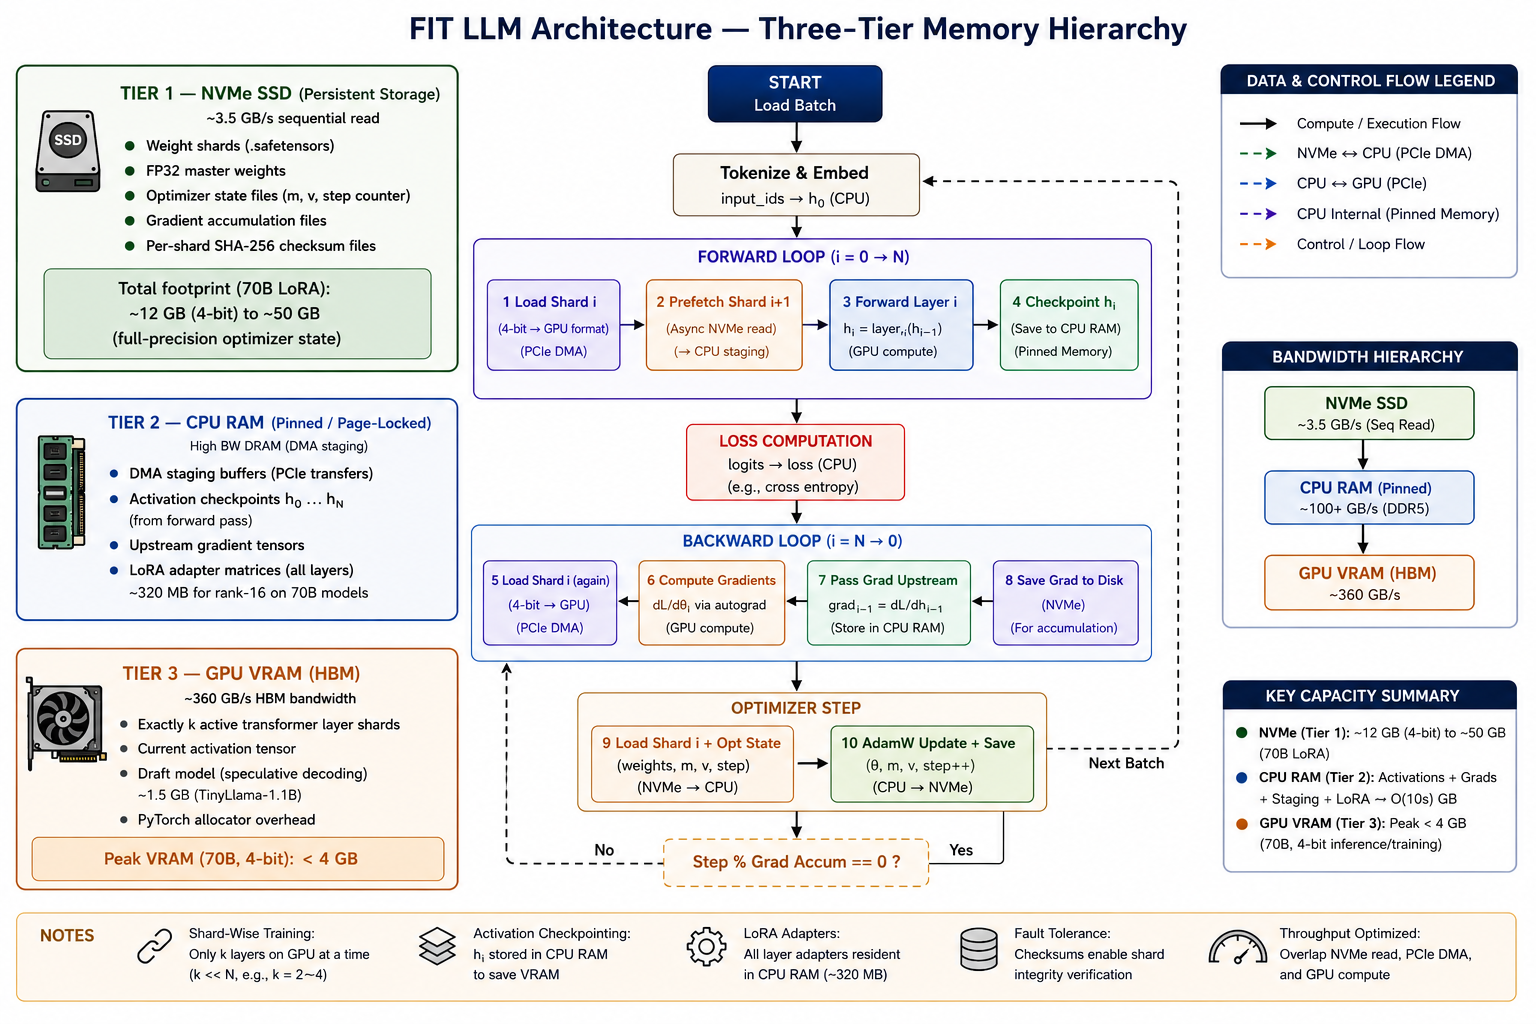
\includegraphics[width=\linewidth]{fig1}
  \caption{FitLLM system architecture across three memory tiers (NVMe SSD $\to$
  CPU RAM $\to$ accelerator VRAM). A hardware profiler feeds the adaptive shard
  scheduler, which drives the forward loop (shards in, activations out to host
  RAM), the reverse-order backward loop (shards reloaded, adapter gradients to
  disk), and the optimizer step. Schematic; any quantities shown are analytical
  design estimates, not measured results.}
  \label{fig:arch}
\end{figure}

\begin{figure}[t]
  \centering
  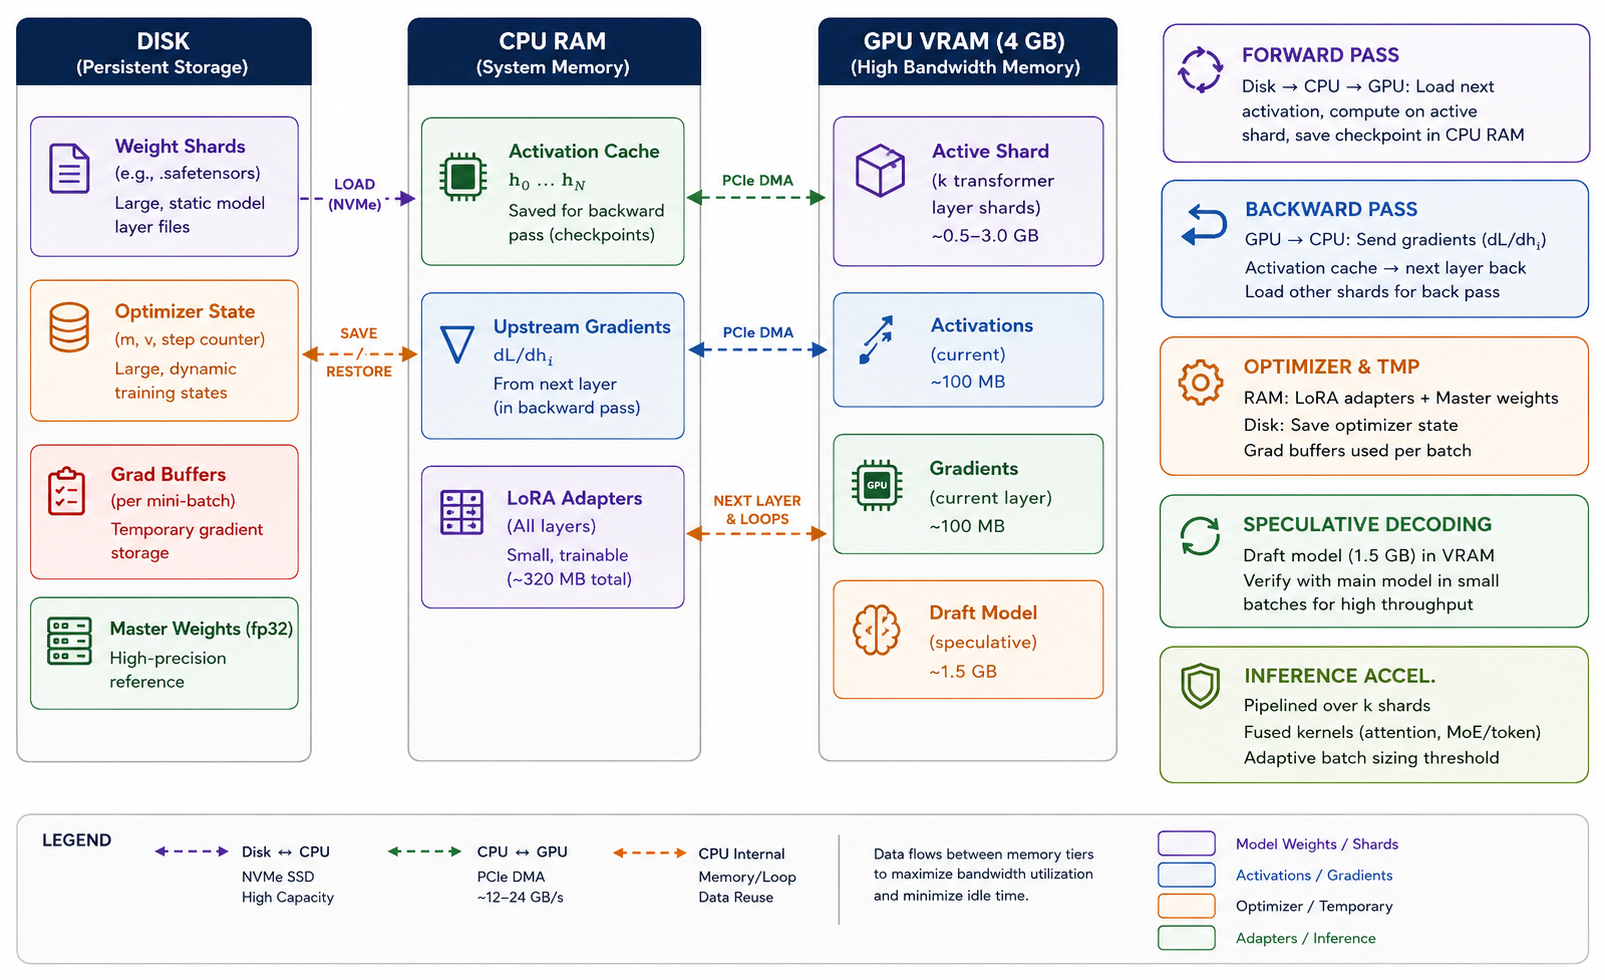
\includegraphics[width=\linewidth]{fig2}
  \caption{Cross-tier dataflow. Weight shards, optimizer state, gradient buffers,
  and master weights reside on disk; an activation cache, upstream gradients, and
  the small LoRA adapters reside in host RAM; a small set of \emph{active} shards,
  current activations and gradients, and an optional draft model reside in
  accelerator VRAM. Arrows mark the forward, backward, optimizer, and speculative
  paths. Schematic illustration.}
  \label{fig:dataflow}
\end{figure}

FitLLM is organised into the components summarised in
Table~\ref{tab:components} and laid out across the three memory tiers of
\autoref{fig:arch}. A control plane (the hardware profiler and shard scheduler)
decides, batch by batch, how much of the model is resident on the accelerator;
a data plane moves shards and activations between tiers. \autoref{fig:dataflow}
shows where each class of tensor lives: the frozen base weights, optimizer state,
gradient buffers, and (in full-parameter mode) \texttt{fp32} master weights stay
on disk; an activation cache, the upstream gradient, and the small trainable
adapters stay in host RAM; and only a small set of \emph{active} shards plus the
current activation/gradient tensors---and, for inference, a lightweight draft
model---ever occupy VRAM.

A model is onboarded once by the sharding step: the host loads the model
(optionally under a $4$-bit quantisation config), the architecture registry
locates its decoder layers, and each layer's state dictionary is written to an
independent shard file with a companion checksum. At execution time the base
model is moved off the accelerator and layers are paged in on demand, so that
peak VRAM is governed by the resident shard width rather than by total model
size.

\begin{table}[t]
  \centering
  \caption{Principal components of FitLLM.}
  \label{tab:components}
  \begin{tabular}{@{}ll@{}}
    \toprule
    \textbf{Component} & \textbf{Responsibility} \\
    \midrule
    Adaptive Shard Probe & Measure live free VRAM/RAM; compute resident shard width $k$; select strategy \\
    Shard Scheduler & Async prefetch pipeline, pinned staging, host weight cache, eviction \\
    Forward Engine & Layer-sequential forward pass; checkpoint activations to host RAM \\
    Backward Engine & Reverse-order shard-wise gradient computation from cached activations \\
    Shard Optimizer & Per-layer (Q)LoRA AdamW update; disk-resident state for full mode \\
    QLoRA Manager & Inject/freeze adapters; route trainable gradients \\
    Accelerated Inference & Speculative decoding + dynamic-$K$ controller + draft KV persistence \\
    Architecture Registry & Map \texttt{model\_type} to layer/embedding/head accessors for $30{+}$ families \\
    Integrity Verifier & SHA-256 at shard creation; verify before deserialisation \\
    Checkpoint Manager & Save/restore adapter weights, optimizer state, data position \\
    \bottomrule
  \end{tabular}
\end{table}

\section{Adaptive Multi-Shard Engine}
\label{sec:amse}

The central control decision is the \emph{resident shard width} $k$: the number
of consecutive decoder layers held on the accelerator at once. Let
$V_{\mathrm{free}}(t)$ be the free accelerator memory measured at step $t$,
$m_{\mathrm{gpu}}$ a safety margin, and $s$ the per-shard size (in the same
units). With analogous host quantities $V^{\mathrm{cpu}}_{\mathrm{free}}$ and
$m_{\mathrm{cpu}}$,
\begin{align}
  k_{\mathrm{gpu}}(t) &= \left\lfloor \frac{V_{\mathrm{free}}(t) - m_{\mathrm{gpu}}}{s} \right\rfloor, &
  k_{\mathrm{cpu}}(t) &= \left\lfloor \frac{V^{\mathrm{cpu}}_{\mathrm{free}}(t) - m_{\mathrm{cpu}}}{s} \right\rfloor, \\
  k(t) &= \min\!\big(k_{\mathrm{gpu}}(t),\, L\big), && \text{if an accelerator is present and } k_{\mathrm{gpu}}(t)>0, \label{eq:k}
\end{align}
where $L$ is the total number of layers. When no accelerator is available or
$k_{\mathrm{gpu}}(t)=0$, the engine sets
$k(t)=\max(1,\min(k_{\mathrm{cpu}}(t),L))$ and routes compute to the host.

\paragraph{Execution strategies.} The probe classifies the current step into one
of four strategies, which downstream engines use to choose code paths:
\emph{full\_model} ($k\!\ge\!L$, the whole model fits and streaming reduces to a
resident execution), \emph{multi\_shard} ($1\!<\!k\!<\!L$, the common case),
\emph{single\_shard} ($k\!=\!1$, minimal footprint), and \emph{cpu\_only}
($k\!=\!0$ on the accelerator, all compute on the host). This taxonomy is what
lets one set of shards serve an $80$\,GB datacentre GPU and a $4$\,GB consumer
GPU without reconfiguration.

\paragraph{Budget enforcement and re-probing.} A user-specified VRAM budget is
enforced by inflating $m_{\mathrm{gpu}}$ so that the \emph{effective} free memory
seen by Eq.~\eqref{eq:k} equals the budget, regardless of the device's physical
capacity. The probe result is cached and re-evaluated every $r$ calls; if $k$
decreases relative to the previous probe, the engine emits a warning, since a
shrinking $k$ signals memory pressure---typically a KV cache that has grown
during long-context decoding. As $V_{\mathrm{free}}(t)$ falls, $k(t)$ decreases
monotonically and, in the limit, later shard batches are routed to the host
instead of triggering an OOM failure. This per-batch re-probing, rather than a
one-time start-up profile, is the distinguishing feature of the AMSE.

\section{Three-Stage Forward Pipeline}
\label{sec:forward}

\begin{figure}[t]
  \centering
  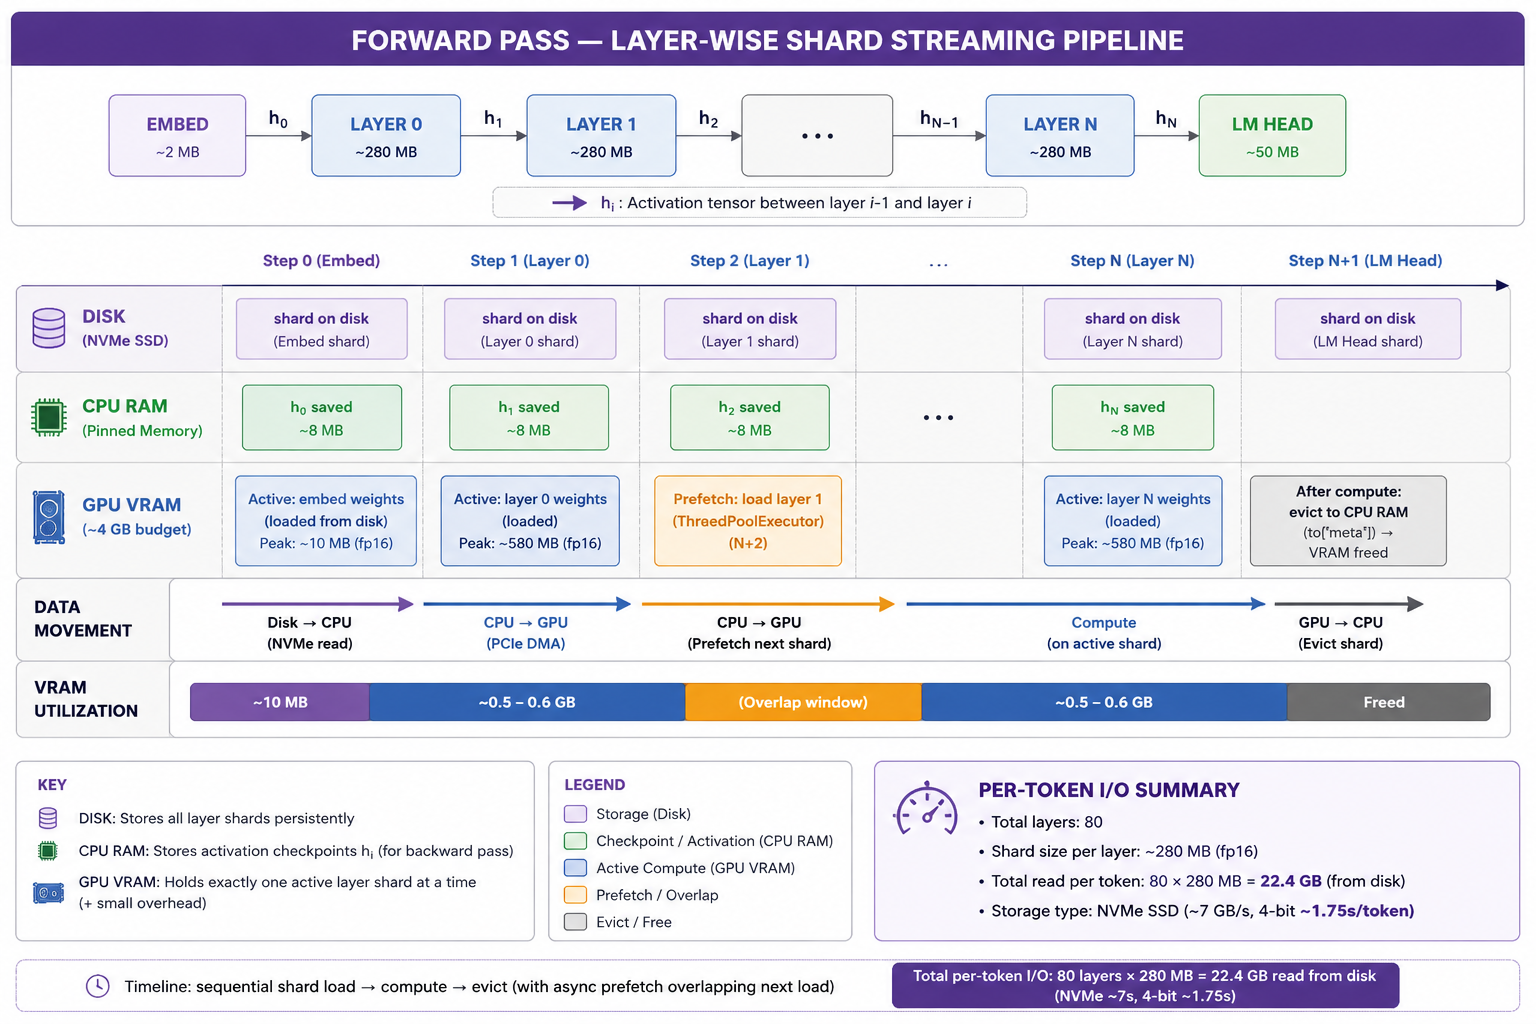
\includegraphics[width=\linewidth]{fig3}
  \caption{Forward pass as a layer-wise shard-streaming pipeline. The embedding
  produces $h_0$; each decoder layer's shard is read from NVMe into pinned host
  RAM, transferred to VRAM, computed, and evicted, while the next batches are
  prefetched and transferred concurrently. Hidden states $h_i$ are written to
  host RAM as activation checkpoints. Schematic; per-token I/O figures shown are
  analytical estimates.}
  \label{fig:forward}
\end{figure}

The forward pass (Algorithm~\ref{alg:forward}, \autoref{fig:forward}) processes
the $L$ layers in $\lceil L/k\rceil$ batches and overlaps three stages across
batches: Stage~A reads the next-but-one batch from NVMe into pinned host RAM;
Stage~B transfers the next batch from host RAM to the accelerator over a
dedicated copy stream; and Stage~C computes the current batch. With perfect
overlap, the wall-clock time per batch approaches
\begin{equation}
  T_{\mathrm{batch}} \;\to\; \max\big(T_{\mathrm{NVMe}},\, T_{\mathrm{PCIe}},\, T_{\mathrm{compute}}\big),
  \label{eq:overlap}
\end{equation}
rather than their sum. After each layer the hidden state $h_i$ is detached and
copied to host RAM as an activation checkpoint for the backward pass, and the
layer's shard is evicted from the accelerator immediately.

\paragraph{Prefetch ordering.} Prefetch requests are issued in descending order
of an exponentially-weighted moving-average (EMA) estimate of each shard's load
time, so the slowest reads are launched first and are least likely to stall the
consumer. The EMA is updated from observed read latencies, adapting to the
storage device and to filesystem-cache warmth.

\paragraph{Heterogeneous placement.} For each batch the engine performs a
headroom check: if free VRAM (after the safety margin) exceeds the shard size by
a small factor, the batch is computed on the accelerator; otherwise it is
computed on the host, with the resulting hidden state transferred forward to the
next accelerator-assigned batch. This per-batch decision (rather than a static
per-layer-type partition) lets a long-context generation continue on the host
once the KV cache has consumed VRAM.

\begin{algorithm}[t]
\caption{Three-stage forward pass}
\label{alg:forward}
\begin{algorithmic}[1]
\State $h \gets \mathrm{embed}(\text{input\_ids})$;\quad save $h$ to host RAM
\State $k \gets \textsc{Probe}()$;\quad start Stage-A prefetch for batches $0$ and $1$
\For{each batch $b$ of $k$ layers}
  \State issue Stage-A prefetch for batch $b{+}2$ \Comment{NVMe $\rightarrow$ host}
  \State collect host tensors for batch $b$; choose compute device by headroom check
  \State Stage-B: async transfer batch $b$ host $\rightarrow$ accelerator
  \For{each layer $i$ in batch $b$}
     \State reconstruct layer $i$ from shard tensors; run $h \gets \mathrm{layer}_i(h)$ under autocast, no-grad
     \State save $h$ to host RAM \Comment{activation checkpoint}
  \EndFor
  \State evict batch $b$ shards from the accelerator
\EndFor
\State \Return $\mathrm{lm\_head}(h)$ and the list of activation checkpoints
\end{algorithmic}
\end{algorithm}

\section{Reverse-Order Shard-Wise Backward Pass}
\label{sec:backward}

\begin{figure}[t]
  \centering
  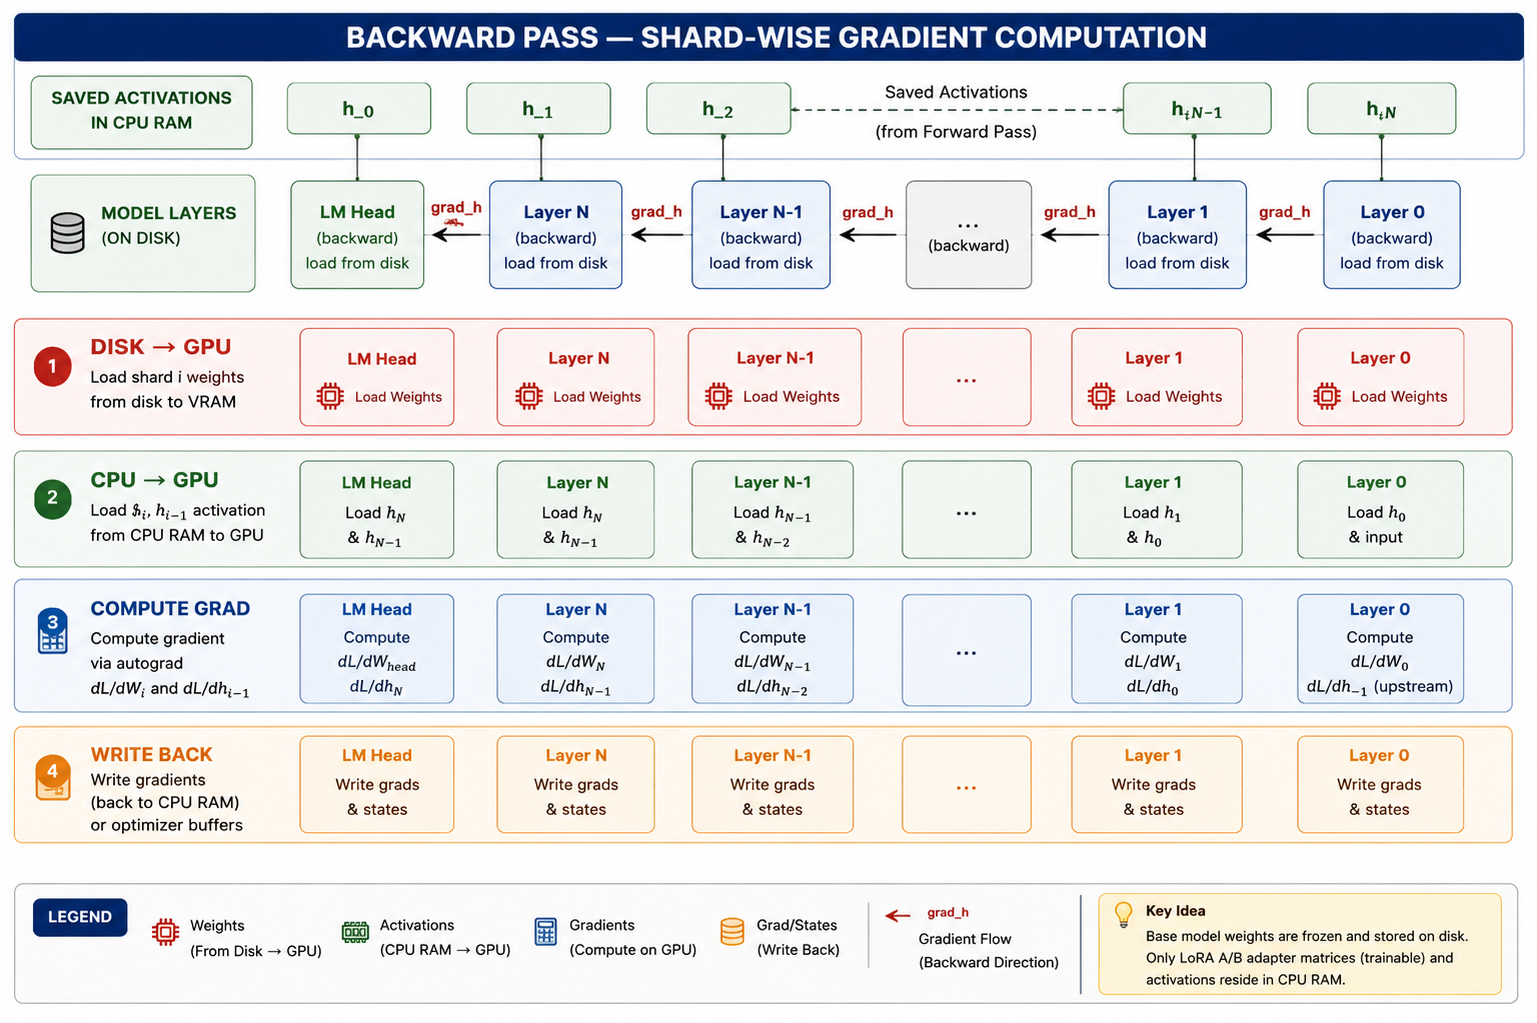
\includegraphics[width=\linewidth]{fig4}
  \caption{Backward pass as reverse-order, shard-wise gradient computation. Using
  the activations saved during the forward pass, each layer is reloaded from disk
  (typically a host-cache hit), recomputed with gradient tracking, and used to
  backpropagate the incoming gradient; only the low-rank adapter gradients are
  written back. The base weights are read-only. Schematic illustration.}
  \label{fig:backward}
\end{figure}

The backward pass (Algorithm~\ref{alg:backward}, \autoref{fig:backward}) never
holds the full computation graph. It first re-runs the language-model head to
obtain the gradient of the loss with respect to the final hidden state. It then
walks the layers in reverse: for layer $i$ it reloads the shard (typically a host
cache hit during fine-tuning), recomputes the layer forward with gradient
tracking on the \emph{checkpointed} input $h_{i-1}$, backpropagates the incoming
gradient $g$ through that single layer to obtain the gradient with respect to
$h_{i-1}$, and accumulates the layer's low-rank adapter gradients to a per-layer
file on disk. The single-layer graph is discarded before the next layer, and the
base weights are treated as read-only.

\begin{algorithm}[t]
\caption{Reverse-order shard-wise backward pass}
\label{alg:backward}
\begin{algorithmic}[1]
\State $h_L \gets$ last activation checkpoint;\quad require grad on $h_L$
\State recompute logits $\gets \mathrm{lm\_head}(h_L)$;\quad $\ell \gets \mathrm{loss}(\text{logits}, y)$
\State $\ell.\mathrm{backward}()$;\quad $g \gets \nabla_{h_L}\ell$ (moved to host)
\For{batch from last to first ($k$ layers at a time)}
  \State prefetch shards for the batch (cache hits during fine-tuning)
  \For{each layer $i$ in the batch, in reverse}
     \State $h_{i-1} \gets$ checkpoint$[i]$; require grad
     \State $h_i \gets \mathrm{layer}_i(h_{i-1})$ with grad tracking
     \State $h_i.\mathrm{backward}(g)$;\quad $g \gets \nabla_{h_{i-1}}$ (to host)
     \State accumulate adapter gradients of layer $i$ to disk
     \State discard the layer graph
  \EndFor
  \State evict the batch shards
\EndFor
\end{algorithmic}
\end{algorithm}

\paragraph{Memory ceiling.} At any instant the accelerator holds at most the $k$
shards of the active batch, the two activation tensors $h_{i-1}$ and $h_i$, and a
bounded working overhead $\varepsilon$. Hence
\begin{equation}
  V_{\mathrm{backward}} \;\le\; k\cdot s_{\mathrm{quant}} \;+\; 2\,a \;+\; \varepsilon,
  \label{eq:ceiling}
\end{equation}
where $s_{\mathrm{quant}}$ is the quantised shard size and $a$ the activation
size. Crucially the bound is \emph{independent of $L$}: deeper models do not
raise the peak accelerator memory of the backward pass, only its duration and its
host-RAM activation footprint. Equation~\eqref{eq:ceiling} is an invariant of the
procedure, not an empirical observation---no other tensors are resident by
construction.

\section{Disk-Resident Optimizer and QLoRA Integration}
\label{sec:optim}

\begin{figure}[t]
  \centering
  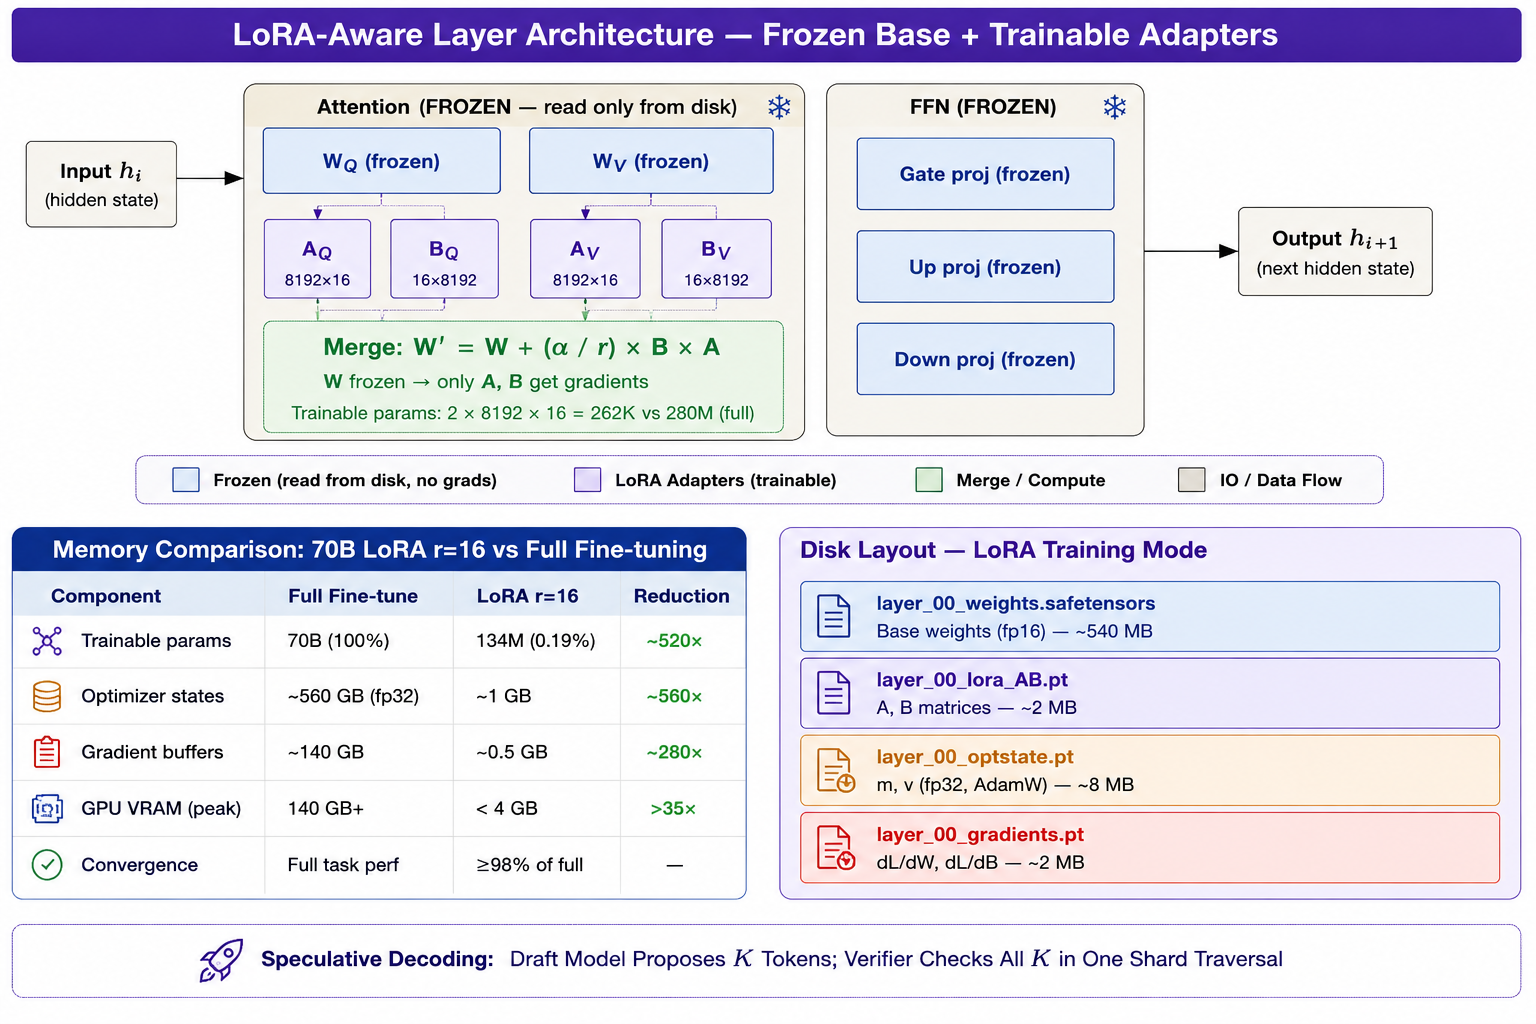
\includegraphics[width=\linewidth]{fig5}
  \caption{LoRA-aware layer architecture and training-mode layout. The base
  attention and MLP projections stay frozen in NF4; trainable low-rank matrices
  $A,B$ are injected with output $W_0 x + (\alpha/r) B(Ax)$. The per-layer file
  bundle stores the quantised weights, an optional \texttt{fp32} master, the
  optimizer moments, and a transient gradient file. Memory-comparison values are
  analytical estimates, not measurements.}
  \label{fig:lora}
\end{figure}

FitLLM wraps the quantised base with QLoRA (\autoref{fig:lora}): the model is
prepared for $k$-bit training (normalisation and head layers cast to
\texttt{fp32}, input gradients enabled) and low-rank $A,B$ adapters are attached
to the attention projections, leaving the NF4 base frozen. For a $32$B model at
rank $16$ this yields $\sim$$33.6$\,M trainable parameters---about $0.10\%$ of the
total---small enough that the adapters and their Adam moments reside comfortably
in host RAM.

\paragraph{Two optimizer modes.} In the default \emph{LoRA} mode the optimizer
keeps moment estimates in host RAM and applies the AdamW update directly to the
live adapter parameters once per accumulation cycle, with no disk traffic for
optimizer state. A separate \emph{full-parameter} mode stores, per layer, an
\texttt{fp32} master copy and the Adam moments as files, loads them on demand,
applies the update, and re-quantises to NF4 after each step; its peak host
requirement is a small constant ($\sim$$3\times$ a single shard's \texttt{fp32}
size) independent of total model size, so even full fine-tuning has no minimum
accelerator-memory requirement. The per-layer file bundle---NF4 weights, optional
\texttt{fp32} master, optimizer moments, transient gradient file, and SHA-256
checksum---is shown on the right of \autoref{fig:lora}.

\paragraph{Host weight cache.} A dynamic host-side cache, sized to free RAM minus
a safety margin with FIFO eviction, retains recently-read shards so that the
backward pass and subsequent micro-batches read from RAM rather than disk; the
cache is invalidated after each optimizer step and re-warmed in the background.

\paragraph{Training schedule.} Training applies a linear-warmup, cosine-decay
learning-rate schedule, global gradient-norm clipping over the adapter
parameters, response-only loss masking for instruction data (the prompt tokens
are excluded from the loss), and periodic checkpointing of adapter weights,
optimizer state, and the data-loader position for exact-step resume.

\section{Speculative Decoding with a Training-Free Dynamic Controller}
\label{sec:spec}

Because each verifier forward pass in a shard-streaming system carries a large
fixed I/O cost, amortising it over several tokens is valuable. FitLLM pairs the
sharded model (verifier) with a small draft model from the same family; tokenizer
compatibility is validated at load time by comparing vocabulary sizes and
spot-checking token-id encodings, since mismatched tokenizers would corrupt the
acceptance test. At each step the draft proposes $K$ tokens using a
\emph{persistent} KV cache; the verifier checks all $K$ in one pass; and tokens
are accepted or rejected by the standard speculative-sampling rule, which
preserves the verifier's distribution (on rejection, a corrected token is sampled
from the residual distribution). A controller maintains a rolling window of
acceptance rates and nudges $K$ within $[K_{\min},K_{\max}]$: high acceptance
raises $K$, low acceptance lowers it---without any auxiliary prediction head or
training. Section~\ref{sec:analysis} analyses the resulting complexity and the
optimal $K$.

\section{First-Principles Analysis}
\label{sec:analysis}

\paragraph{Optimal shard width vs.\ context length.}
Let $V_{\mathrm{total}}$ be the budget, $V_{\mathrm{ovh}}$ fixed overhead, and
$V_{\mathrm{KV}}(t)$ the KV-cache size after $t$ tokens. The largest admissible
shard width is
\begin{equation}
  k^\star(t) = \left\lfloor \frac{V_{\mathrm{total}} - V_{\mathrm{ovh}} - V_{\mathrm{KV}}(t)}{s_w} \right\rfloor,
  \qquad
  V_{\mathrm{KV}}(t) \approx \frac{t \cdot n_{\mathrm{kv}} \cdot d_{\mathrm{head}} \cdot 2 \cdot \mathrm{bytes}}{10^9}.
  \label{eq:kstar}
\end{equation}
For a $70$B-class model in $4$-bit ($s_w\!\approx\!0.135$\,GB) under an $8$\,GB
budget, Eq.~\eqref{eq:kstar} gives $k^\star\!\approx\!53$ at $t=0$ and
$k^\star\!\to\!0$ as $t$ grows, at which point the engine switches to host
execution. These are analytical estimates from
Eqs.~\eqref{eq:k}--\eqref{eq:kstar}, not measurements.

\paragraph{Backward-pass memory budget.}
Table~\ref{tab:budget} instantiates the ceiling of Eq.~\eqref{eq:ceiling} and the
host/disk footprints for a $70$B model at LoRA rank $16$, illustrating that the
accelerator term is governed by $k$ and the two activation tensors while the bulk
of the model rests on disk. All values are analytical.

\begin{table}[t]
  \centering
  \caption{Analytical memory budget across tiers for a $70$B model, LoRA rank
  $16$ (illustrative; not measured). The accelerator footprint follows
  Eq.~\eqref{eq:ceiling} and is independent of model depth.}
  \label{tab:budget}
  \begin{tabular}{@{}lll@{}}
    \toprule
    \textbf{Tier} & \textbf{Contents} & \textbf{Scaling} \\
    \midrule
    NVMe disk & NF4 base shards; \texttt{fp32} master (full mode); optimizer state; transient grads & $O(\text{model size})$ \\
    Host RAM & activation checkpoints; upstream gradient; LoRA adapters + Adam moments & $O(L \cdot a) + O(\text{adapters})$ \\
    Accelerator & $k$ active shards $+\,2$ activation tensors $+\,\varepsilon$ & $k\,s_{\mathrm{quant}} + 2a$ \\
    \bottomrule
  \end{tabular}
\end{table}

\paragraph{Draft complexity with KV persistence.}
Without a persistent draft cache, generating $n$ draft tokens re-encodes a growing
prefix and costs $1+2+\dots+n = n(n{+}1)/2 = O(n^2)$ draft forward units; with
persistence each token costs one unit, for $O(n)$ total. The ratio at $n=200$ is
$(200\cdot 201/2)/200 = 100.5\times$ (exact arithmetic for the draft path only).

\paragraph{Optimal draft length.}
With per-token acceptance probability $\alpha$, verifier cost $T_v$, and draft
cost $T_d$, the expected tokens-per-second of speculative decoding is
\begin{equation}
  \mathrm{TPS}(K) = \frac{1-\alpha^{K+1}}{(1-\alpha)\,(T_v + K\,T_d)}.
  \label{eq:tps}
\end{equation}
In the shard-streaming regime $T_v \gg T_d$, so the optimum is pushed toward
$K_{\max}$ unless $\alpha$ is small; the rolling controller of
Section~\ref{sec:spec} tracks $K^\star(t)$ implicitly without knowing
$T_v,T_d$.

\paragraph{Roofline rationale for heterogeneous placement.}
At decode time the effective batch size is $1$, so every layer type is
memory-bandwidth bound (arithmetic intensity below the device's critical
intensity $b_{\mathrm{crit}}=\text{peak\,FLOP/s}/\text{bandwidth}$). The per-layer
time ratio between accelerator and host is then approximately the
memory-bandwidth ratio (commonly $\sim$$7\times$), so the accelerator is preferred
whenever it has headroom; when VRAM is exhausted by the KV cache, host execution
is still preferable to OOM or to repeated NVMe reloads. FitLLM therefore fills the
accelerator first and degrades to the host, rather than statically partitioning
layers across tiers.

\section{Implementation}
\label{sec:impl}

FitLLM is implemented in Python on PyTorch, using \texttt{safetensors} for
shards, \texttt{bitsandbytes} for NF4 quantisation, and PEFT for LoRA.
Asynchronous I/O is provided by a bounded thread pool with a pinned-buffer
semaphore and a dedicated CUDA copy stream.

\paragraph{Architecture registry.} A registry maps a model's \texttt{model\_type}
string to the dotted attribute paths of its decoder layers, token embedding, and
output head, covering $30{+}$ dense and mixture-of-experts families
(e.g.\ \textsc{llama}, \textsc{qwen2/3}, \textsc{mistral}, \textsc{gemma},
\textsc{phi}, \textsc{falcon}, \textsc{gpt2}, \textsc{mixtral},
\textsc{deepseek}), with a heuristic fallback for unknown types. This enables
zero-config onboarding directly from a checkpoint, without model instantiation
or format conversion.

\paragraph{Acceleration stack.} Beyond the streaming substrate, FitLLM layers
several orthogonal accelerations on the resident shards, each chosen so that it
composes with the others: (1) $4$-bit NF4 block-wise compression of the base
weights, cutting disk and transfer volume $\sim$$4\times$; (2) double-buffered
prefetch ($k{+}2$ look-ahead) to hide NVMe latency; (3) pinned host buffers and
CUDA streams so PCIe transfers overlap compute; (4) fused kernels
(FlashAttention~\citep{dao2022flashattention}, fused RMSNorm/MLP) on resident
layers; (5) speculative decoding (Section~\ref{sec:spec}); (6) adaptive layer
skipping that elides a layer when the cosine similarity between successive hidden
states exceeds a threshold; and (7) \texttt{mmap}/OS-page-cache-backed shard
reads so that warm reruns avoid disk entirely. These are design mechanisms; the
per-technique factors are analytical and are not claimed as measured speedups.

\paragraph{Integrity and resumption.} Each shard is written with a SHA-256
checksum that is verified before deserialisation, and a \texttt{verify} command
re-checks an entire shard directory and names any corrupted file. The checkpoint
manager saves adapter weights, optimizer state, and the data-loader position for
exact-step resume. A command-line interface exposes \texttt{shard},
\texttt{generate}, \texttt{train}, \texttt{probe}, and \texttt{verify}
subcommands, and all settings are configurable via environment variables or a
\texttt{.env} file.

\section{Feasibility Evaluation}
\label{sec:eval}

We evaluate \emph{memory feasibility}---the central claim that a model far larger
than the VRAM budget can be sharded and executed, forward and backward, within
that budget---rather than end-to-end throughput or downstream quality, which we
address as future work in Section~\ref{sec:limitations}.

\paragraph{Setup.} We shard \textsc{Qwen2.5-32B-Instruct} ($32.8$B parameters)
with NF4 double quantisation and attach rank-$16$ QLoRA adapters to the
$\{q,k,v,o\}$ projections. The accelerator working set is constrained to $4$\,GB
through the budget mechanism of Section~\ref{sec:amse} (by inflating the safety
margin so the probe sees only $4$\,GB of effective free memory), independent of
the physical device capacity. Fine-tuning uses the Alpaca instruction dataset
with response-only loss masking, sequence length $512$, and gradient
accumulation.

\paragraph{Results.} Table~\ref{tab:feasibility} reports the measured static
quantities. The $32$B base is materialised as $64$ per-layer shards totalling
$\sim$$15.5$\,GB on disk ($\sim$$242$\,MB per shard), none of which need be
resident in full on any single tier. QLoRA exposes $33{,}554{,}432$ trainable
parameters, $0.10\%$ of the total, with adapter-plus-optimizer checkpoints of
$\sim$$0.4$\,GB. Under the $4$\,GB budget the probe admits roughly $13$ resident
layers per batch, and the forward and reverse-order backward passes of
Sections~\ref{sec:forward}--\ref{sec:backward} complete within the budget on a
single accelerator, with activation checkpoints held in host RAM and base weights
streamed from disk. This confirms the construction's memory invariants in
practice: peak accelerator memory tracks the resident shard width and the two
activation tensors of Eq.~\eqref{eq:ceiling}, not model depth.

\begin{table}[t]
  \centering
  \caption{Feasibility measurements for \textsc{Qwen2.5-32B-Instruct} under a
  $4$\,GB accelerator working-set budget.}
  \label{tab:feasibility}
  \begin{tabular}{@{}lr@{}}
    \toprule
    \textbf{Quantity} & \textbf{Value} \\
    \midrule
    Base parameters & $3.28\times10^{10}$ \\
    Quantisation & NF4 (double-quant) \\
    Decoder layers / shards & $64$ \\
    Per-shard size & $\sim$$242$\,MB \\
    Total shard footprint on disk & $\sim$$15.5$\,GB \\
    Trainable (LoRA, rank $16$) parameters & $3.36\times10^{7}$ \\
    Trainable fraction & $0.10\%$ \\
    Resident layers per batch ($4$\,GB budget) & $\sim$$13$ \\
    Adapter\,+\,optimizer checkpoint size & $\sim$$0.4$\,GB \\
    \bottomrule
  \end{tabular}
\end{table}

\section{Limitations and Future Work}
\label{sec:limitations}

The present prototype establishes memory feasibility and the analytical
properties above, but does not yet demonstrate competitive end-to-end throughput
or validated convergence at scale, and we are explicit about this.

\paragraph{Throughput.} In its current form, each training step re-reads and
re-hashes the full shard set when per-shard integrity verification is left
enabled, and performs aggressive per-layer memory reclamation (garbage collection
and allocator trimming) after every layer. These safety mechanisms dominate the
step time and place the prototype far from the overlap upper bound of
Eq.~\eqref{eq:overlap}. The mitigations are straightforward and are the focus of
ongoing work: verify checksums once at load rather than per pass, batch or
amortise eviction, retain the host weight cache across accumulation cycles, and
exploit direct NVMe-to-accelerator DMA where the topology allows. We report these
honestly rather than presenting tuned throughput numbers the prototype does not
yet achieve.

\paragraph{Numerical fidelity.} Faithful fine-tuning through reconstructed,
quantised layers requires that the recomputed backward exactly mirror the
forward---identical attention masking, positional encodings, and compute
precision---and that quantisation state round-trips through sharding without
loss. Hardening this equivalence, and reporting loss curves and downstream task
metrics against an in-memory QLoRA baseline, is the most important item of future
work; we therefore make no quality claims here.

\paragraph{Scope.} The analyses target dense decoder-only transformers;
mixture-of-experts models are supported structurally by the registry but their
expert-aware sharding and placement are not analysed here.

\section{Conclusion}
\label{sec:conclusion}

We presented FitLLM, a single-device system that executes inference and low-rank
fine-tuning of large dense transformers within a fixed, user-specified
accelerator-memory budget by streaming per-layer disk shards through an adaptive
three-tier pipeline. The design provides an out-of-memory-free execution model
via continuous re-probing and graceful CPU fallback, and a reverse-order backward
pass whose accelerator memory is provably independent of model depth. We
demonstrated that a $32$B model fits and executes within a $4$\,GB working set
while training only $0.10\%$ of its parameters, and we gave first-principles
analyses of shard width, the backward-pass memory ceiling, and the
speculative-decoding path. Closing the gap between memory feasibility and
production throughput---primarily by amortising integrity and reclamation
overheads and validating numerical fidelity end to end---is the natural next
step.

\bibliographystyle{plainnat}
\begin{thebibliography}{10}
\providecommand{\natexlab}[1]{#1}

\bibitem[Aminabadi et al.(2022)]{aminabadi2022deepspeed}
R.~Y. Aminabadi, S.~Rajbhandari, A.~A. Awan, C.~Li, D.~Li, E.~Zheng, O.~Ruwase,
  S.~Smith, M.~Zhang, J.~Rasley, and Y.~He.
\newblock {DeepSpeed-Inference}: Enabling efficient inference of transformer
  models at unprecedented scale.
\newblock In \emph{SC22: International Conference for High Performance Computing,
  Networking, Storage and Analysis}, 2022.

\bibitem[Chen et al.(2023)]{chen2023accelerating}
C.~Chen, S.~Borgeaud, G.~Irving, J.-B. Lespiau, L.~Sifre, and J.~Jumper.
\newblock Accelerating large language model decoding with speculative sampling.
\newblock \emph{arXiv preprint arXiv:2302.01318}, 2023.

\bibitem[Dao et al.(2022)]{dao2022flashattention}
T.~Dao, D.~Y. Fu, S.~Ermon, A.~Rudra, and C.~R{\'e}.
\newblock {FlashAttention}: Fast and memory-efficient exact attention with
  {IO}-awareness.
\newblock In \emph{Advances in Neural Information Processing Systems (NeurIPS)}, 2022.

\bibitem[Dettmers et al.(2023)]{dettmers2023qlora}
T.~Dettmers, A.~Pagnoni, A.~Holtzman, and L.~Zettlemoyer.
\newblock {QLoRA}: Efficient finetuning of quantized {LLM}s.
\newblock In \emph{Advances in Neural Information Processing Systems (NeurIPS)}, 2023.

\bibitem[Hu et al.(2022)]{hu2022lora}
E.~J. Hu, Y.~Shen, P.~Wallis, Z.~Allen-Zhu, Y.~Li, S.~Wang, L.~Wang, and W.~Chen.
\newblock {LoRA}: Low-rank adaptation of large language models.
\newblock In \emph{International Conference on Learning Representations (ICLR)}, 2022.

\bibitem[Leviathan et al.(2023)]{leviathan2023speculative}
Y.~Leviathan, M.~Kalman, and Y.~Matias.
\newblock Fast inference from transformers via speculative decoding.
\newblock In \emph{International Conference on Machine Learning (ICML)}, 2023.

\bibitem[Ren et al.(2021)]{ren2021zerooffload}
J.~Ren, S.~Rajbhandari, R.~Y. Aminabadi, O.~Ruwase, S.~Yang, M.~Zhang, D.~Li,
  and Y.~He.
\newblock {ZeRO-Offload}: Democratizing billion-scale model training.
\newblock In \emph{USENIX Annual Technical Conference (ATC)}, 2021.

\bibitem[Sheng et al.(2023)]{sheng2023flexgen}
Y.~Sheng, L.~Zheng, B.~Yuan, Z.~Li, M.~Ryabinin, B.~Chen, P.~Liang, C.~R{\'e},
  I.~Stoica, and C.~Zhang.
\newblock {FlexGen}: High-throughput generative inference of large language
  models with a single {GPU}.
\newblock In \emph{International Conference on Machine Learning (ICML)}, 2023.

\end{thebibliography}

\end{document}
